\section{File System}
Il file system é una parte del sistema operativo che si occupa di organizzare i file all'interno dei dischi

\subsection{I File}
Sono l'elemento principale per la maggior parte delle applicazioni, molto spesso, l'input di un' applicazione é un file;
quasi altrettanto spesso, l'output é un file, i file sopravvivono ai processi, il file system é una delle parti del sisema operativo che
sono piú importanti per l'utente, le propietá che il SO deve gesitre sono :
\begin{itemize}
    \item i file devono esistere a lungo termine
    \item condivisibilitá con altri processi (tramite nome simbolici)
    \item strutturabilitá (directory gerarchiche)
\end{itemize}
\subsubsection*{Gestione dei file}
I file sono gestiti da un insieme di programmi e librerie di utilitá, tali programmi sono gestiti in kernel mode, li
librerie vengono invocate come system call, ed hanno a che fare soprattuto con la memoria secondaria, inoltre
in linux é possibile gestire porzioni di RAM come se foessero file, Forniscono un'astrazionie sotto forma di operazionit tipiche
per ogni file vengono mantenuti degli attributi tipo nome permessi \ldots
\subsubsection*{Operazioni sui file}
\begin{itemize}
    \item Creazione (con annessa scelta del nome)
    \item Cancellazzione
    \item Apertura
    \item Lettura
    \item Scrittura
    \item Chiusura
\end{itemize}
le operazioni di dlettura é scrittura sono possibili solo se il file é stato aperto
\subsubsection*{Terminologia}
\begin{itemize}
    \item Campo (field)
    \item Record
    \item File
    \item Data Base
\end{itemize}
\subsubsection*{Campi}
\begin{itemize}
    \item dati di base
    \item contengono valori singoli
    \item caratterizzati da lunghezza e tipo di dato (o demarcazioni)
    \item esempio tipico: ASCII
\end{itemize}
\subsubsection*{Record}
\begin{itemize}
    \item Insieme di campi
    \item ognuno trattato come un'unitá
\end{itemize}
\subsubsection*{File}
\begin{itemize}
    \item Hanno un nome
    \item Sono insiemi di record correlati in ogni file ogni record é un solo campo con un byte
    \item Ogni file é trattato come unitá con nome propio
    \item possono implementare meccanismi di controllo di accesso
\end{itemize}
\subsubsection*{DataBase}
\begin{itemize}
    \item Sono un'opportuna collezione di file
    \item sono gestiti dai DBMS che sono processi di un sistema operativo
    \item Nei system operativi moderni non é piú necessario gestire File attraverso i data base
\end{itemize}
\subsubsection*{Sistemi per la gestione di file}
    \begin{figure}[H]
    \centering
    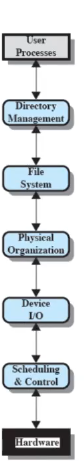
\includegraphics[width=0.2\textwidth]{immagini/FileSystemIO}
\end{figure}
I file managements Systems forniscono servizi agli utenti e alle applicazioni per l'uso di file e definiscono anche il modo in cui i
file sono usati, sollevando i programmatori dal dover scrivere codice per gestire i file
\subsection{Obbiettivi per il File Management Systems}
\begin{itemize}
    \item Rispondere alle necessita degli utenti riguardo alla gestione dei dati
    \item Garantire che i dati nei file siano validi
    \item Ottimizzare le prestazioni : sia dal punto di vista di throughput che tempo di risposta
    \item Fornire supporto per diversi tipi di memoria secondari
    \item minimizzare i dati per o distrutti
    \item Fornire un insieme di interfacce standard per i processi utente
    \item Fornire supporto per l'I/O effettuato da piú utenti in contemporaneamente
\end{itemize}
\subsubsection*{Requisiti}
\begin{enumerate}
    \item Ogni utente deve essere in grado di creare, cancellarem, leggere, scrivere e modificare un file
    \item Ogni utente deve poter accedere, in modo controllato, ai file di un altro utente
    \item Ogni utente deve poter leggere e modificare i permessi di accesso ai propri file
    \item Ogni utente deve poter ristrutturare i propri file in modo attinente al problema affrontato
    \item Ogni utente deve poter muovere dati da un file ad un altro
    \item Ogni utente deve poter mantenere una cop9ia di backup dei propri file (in caso di danno)
    \item Ogni utente deve poter accedere ai propri file tramite nomi simbolici
\end{enumerate}
